\documentclass{beamer}
\usepackage{beamerthemesplit}
\usepackage{subfig}
\usepackage{amssymb,amsmath,mathtools}
\usepackage{amsfonts,booktabs}
\usepackage{lmodern,textcomp}
\usepackage{color}
\usepackage{tikz}
\usepackage{natbib}
\usepackage{multicol}
\usepackage{ctex}
\usepackage[level]{datetime}
\usepackage{listings}


\usetheme{Warsaw}
\newdateformat{ukdate}{\monthname[\THEMONTH] \ordinaldate{\THEDAY} , \THEYEAR}
\lstset{
 columns=fixed,       
 numbers=left,                                        % 在左侧显示行号
 numberstyle=\tiny\color{gray},                       % 设定行号格式
 frame=none,                                          % 不显示背景边框
 backgroundcolor=\color[RGB]{245,245,244},            % 设定背景颜色
 keywordstyle=\color[RGB]{40,40,255},                 % 设定关键字颜色
 numberstyle=\footnotesize\color{darkgray},           
 commentstyle=\it\color[RGB]{0,96,96},                % 设置代码注释的格式
 stringstyle=\rmfamily\slshape\color[RGB]{128,0,0},   % 设置字符串格式
 showstringspaces=false,                              % 不显示字符串中的空格
 language=c++,                                        % 设置语言
}


\title{基于生成式先验的人像视频编辑}
\author{汪兆辰}
\date{\ukdate\today}

\begin{document}

\begin{frame}
    \titlepage
\end{frame}

\section{前端页面}

\begin{frame}
    % 前端页面截图
\end{frame}

\section{后端业务逻辑}

\begin{frame}
    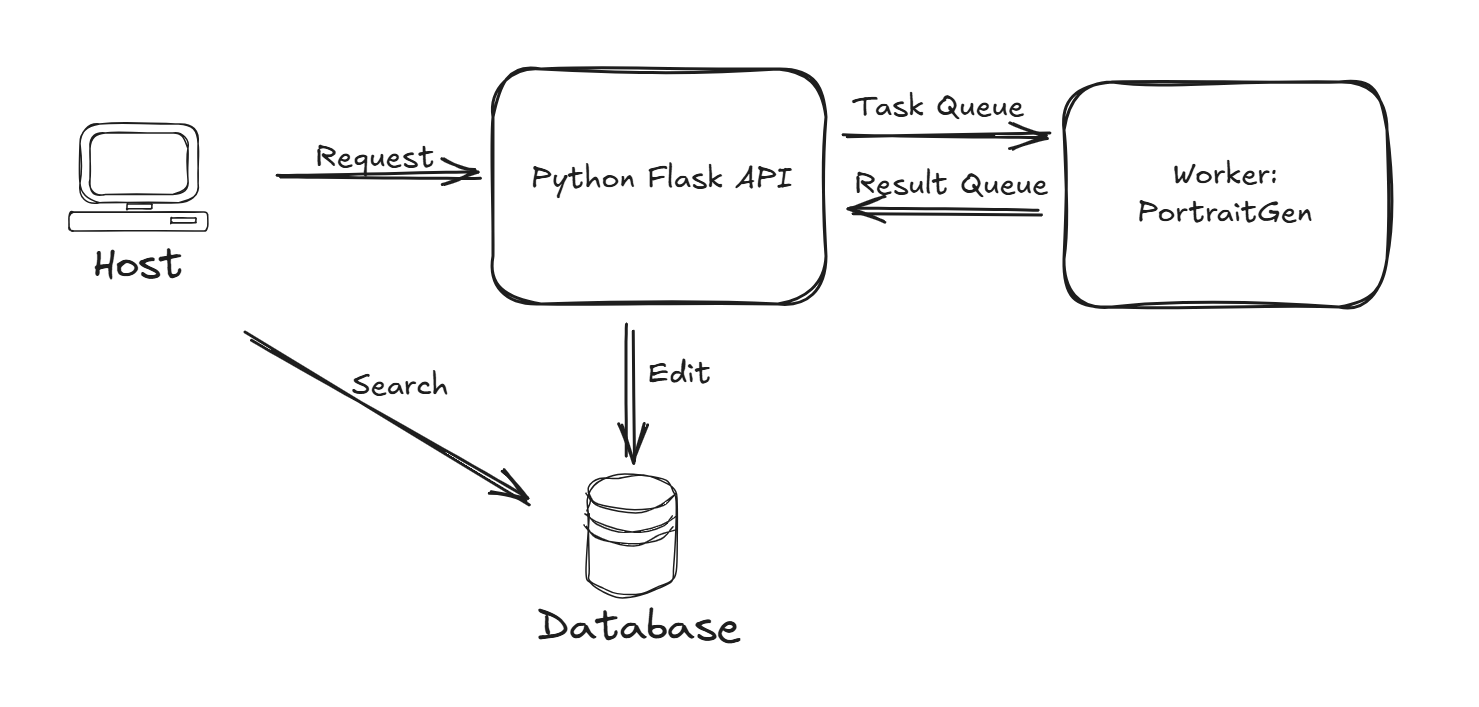
\includegraphics[width=0.9\textwidth]{pic1.png}
    \begin{itemize}
        \item 前端采用Next.js框架搭建页面,后端使用Python的Flask框架搭建API,数据库采用MySQL与Redis
        \item 前端实现用户的视频与Prompt上传,向API发送请求后通过Redis构建任务队列管理并发,在

    \end{itemize}

\end{frame}

\end{document}